\newpage
\section{CPU Scheduling}
\subsection{Basic Concepts}
Maximum CPU utilization obtained with multiprogramming. 

CPU---I/O Burst Cycle
\begin{figure}[!htb]
    \centering
    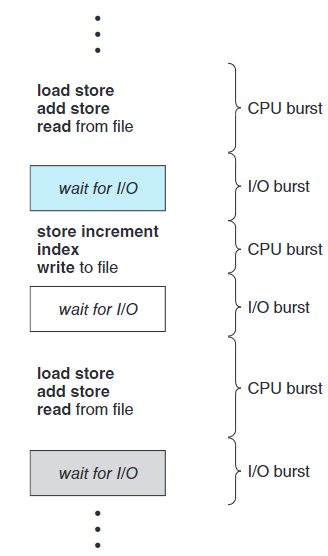
\includegraphics[width=0.22\textwidth]{pic/OS5/Alternating sequence of CPU and IO bursts}
    \caption{Alternating sequence of CPU and I/O bursts}
\end{figure}
CPU bursts 远短于 I/O bursts. CPU bursts time 大致在都在 8ms 以内.  

\subsubsection{CPU Scheduler}
CPU scheduling decisions may take place when a process:
\begin{enumerate}
    \item switches from the running state to the waiting state
    \item switches from the running state to the ready state 
    \item switches from the waiting state to the ready state
    \item terminates
\end{enumerate}
Scheduling under 1 and 4 is non-preemptive. All other scheduling is preemptive. 

\subsubsection{Dispatcher}
involves:
\begin{itemize}
    \item switching context
    \item switching to user mode
    \item jumping to the proper location in the user program to restart that program
\end{itemize}

\begin{figure}[!htb]
    \centering
    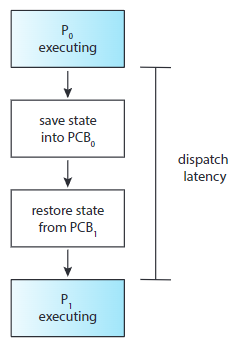
\includegraphics[width=0.22\textwidth]{pic/OS5/The role of the dispatcher}
    \caption{The role of the dispatcher}
\end{figure}

\subsection{Scheduling Criteria}
\begin{itemize}\small
    \item CPU utilization (CPU利用率)--- keep the CPU as busy as possible
    \item Throughput (吞吐率)--- \# of processes that complete their execution per time unit
    \item Turnaround time (周转时间)--- amount of time to execute a particular process
    \item Waiting time (等待时间)--- amount of time a process has been waiting in the \textbf{ready queue} (不算 I/O 时 的时间)
    \item Response time (响应时间)--- amount of time it takes from when a request was submitted until the first response is produced, not output (for time-sharing environment)
\end{itemize}

\subsubsection{Optimization Criteria} 
\begin{itemize}\small
    \item Max CPU utilization
    \item Max throughput
    \item Min turnaround time
    \item Min waiting time
    \item Min response time
\end{itemize}

\subsection{Scheduling Algorithms}
The Gantt Chart

\subsubsection{First-Come, First-Served (FCFS) Scheduling}

\begin{table}[!htb]
    \centering
    % \caption{FCFS Scheduling}
    \begin{tabular}[c]{cc}\toprule
        Process & Burst Time \\ \midrule
        $P_1$ & 24 \\
        $P_2$ & 3 \\
        $P_3$ & 3 
        \\ \bottomrule
    \end{tabular}
\end{table}

\begin{enumerate}
    \item Suppose that the processes arrive in the order: $P_1, P_2, P_3$
    \begin{figure}[!htb]
        \centering
        \tikzmath{
            \s1=0; 
            \s2=0.8*8; 
            \s3=\s2+0.8;
            \s4=\s3+0.8;
            \h=0.8;
        } 
        \begin{tikzpicture}
            \path[draw=black] (\s1,0) rectangle (\s2,\h);
            \path[draw=black] (\s2,0) rectangle (\s3,\h);
            \path[draw=black] (\s3,0) rectangle (\s4,\h);
    
            \node at (\s1/2 + \s2/2, \h/2) {$P_1$};
            \node at (\s2/2 + \s3/2, \h/2) {$P_2$};
            \node at (\s3/2 + \s4/2, \h/2) {$P_3$};
    
            \node at (\s1, -\h/2) {0};
            \node at (\s2, -\h/2) {24};
            \node at (\s3, -\h/2) {27};
            \node at (\s4, -\h/2) {30};
        \end{tikzpicture}
        \caption{FCFS Scheduling Example 1}
    \end{figure}
    \subitem Average waiting time: $(0+24+27)/3=17$
    \item Suppose that the processes arrive in the order: $P_2, P_3, P_1$
    \begin{figure}[!htb]
        \centering
        \tikzmath{
            \s1=0; 
            \s2=0.8; 
            \s3=\s2+0.8;
            \s4=\s3+0.8*8;
            \h=0.8;
        } 
        \begin{tikzpicture}
            \path[draw=black] (\s1,0) rectangle (\s2,\h);
            \path[draw=black] (\s2,0) rectangle (\s3,\h);
            \path[draw=black] (\s3,0) rectangle (\s4,\h);
    
            \node at (\s1/2 + \s2/2, \h/2) {$P_2$};
            \node at (\s2/2 + \s3/2, \h/2) {$P_3$};
            \node at (\s3/2 + \s4/2, \h/2) {$P_1$};
    
            \node at (\s1, -\h/2) {0};
            \node at (\s2, -\h/2) {3};
            \node at (\s3, -\h/2) {6};
            \node at (\s4, -\h/2) {30};
        \end{tikzpicture}
        \caption{FCFS Scheduling Example 2}
    \end{figure}
    \subitem Average waiting time: $(6+0+3)/3=3$
\end{enumerate}
Convoy effect short process behind long process. 

\subsubsection{Shortest-Job-First (SJF) Scheduling}
与 进程 的 burst time 长度相关, 选取长度最小的 进程. 

SJF 是平均等待时间最优的算法, 但缺点是需要知道所有进程的 burst time, 这几乎不可能. 

\begin{table}[!htb]
    \centering
    % \caption{}
    \begin{tabular}[c]{ccc}\toprule
        Process & Arrival Time & Burst Time \\ \midrule
        $P_1$ & 0 & 7 \\
        $P_2$ & 2 & 4 \\
        $P_3$ & 4 & 1 \\
        $P_4$ & 5 & 4 \\
        \bottomrule
    \end{tabular}
\end{table}

\paragraph{Example of Non-Preemptive SJF}进程不能被打断
\begin{figure}[!htb]
    \centering
    \tikzmath{
        \step=0.5;
        \s1=0; 
        \s2=\step*7; 
        \s3=\s2+\step;
        \s4=\s3+\step*4;
        \s5=\s4+\step*4;
        \h=0.8;
    } 
    \begin{tikzpicture}
        \path[draw=black] (\s1,0) rectangle (\s2,\h);
        \path[draw=black] (\s2,0) rectangle (\s3,\h);
        \path[draw=black] (\s3,0) rectangle (\s4,\h);
        \path[draw=black] (\s4,0) rectangle (\s5,\h);

        \node at (\s1/2 + \s2/2, \h/2) {$P_1$};
        \node at (\s2/2 + \s3/2, \h/2) {$P_3$};
        \node at (\s3/2 + \s4/2, \h/2) {$P_2$};
        \node at (\s4/2 + \s5/2, \h/2) {$P_4$};

        \node at (\s1, -\h/2) {0};
        \node at (\s2, -\h/2) {7};
        \node at (\s3, -\h/2) {8};
        \node at (\s4, -\h/2) {12};
        \node at (\s5, -\h/2) {16};
    \end{tikzpicture}
    \caption{Non-Preemptive SJF Example}
\end{figure}

Average waiting time$= (0 + 6 + 3 + 7)/4 = 4$\\
(arrival $\to$ start running) 

\paragraph{Example of Preemptive SJF}进程可以被打断
\begin{figure}[!htb]
    \centering
    \tikzmath{
        \step=0.5;
        \s1=0; 
        \s2=\step*2; 
        \s3=\s2+\step*2;
        \s4=\s3+\step*1;
        \s5=\s4+\step*2;
        \s6=\s5+\step*4;
        \s7=\s6+\step*5;
        \h=0.8;
    } 
    \begin{tikzpicture}
        \path[draw=black] (\s1,0) rectangle (\s2,\h);
        \path[draw=black] (\s2,0) rectangle (\s3,\h);
        \path[draw=black] (\s3,0) rectangle (\s4,\h);
        \path[draw=black] (\s4,0) rectangle (\s5,\h);
        \path[draw=black] (\s5,0) rectangle (\s6,\h);
        \path[draw=black] (\s6,0) rectangle (\s7,\h);

        \node at (\s1/2 + \s2/2, \h/2) {$P_1$};
        \node at (\s2/2 + \s3/2, \h/2) {$P_2$};
        \node at (\s3/2 + \s4/2, \h/2) {$P_3$};
        \node at (\s4/2 + \s5/2, \h/2) {$P_2$};
        \node at (\s5/2 + \s6/2, \h/2) {$P_4$};
        \node at (\s6/2 + \s7/2, \h/2) {$P_1$};

        \node at (\s1, -\h/2) {0};
        \node at (\s2, -\h/2) {2};
        \node at (\s3, -\h/2) {4};
        \node at (\s4, -\h/2) {5};
        \node at (\s5, -\h/2) {7};
        \node at (\s6, -\h/2) {11};
        \node at (\s7, -\h/2) {16};
    \end{tikzpicture}
    \caption{Non-Preemptive SJF Example}
\end{figure}

Average waiting time $= (9 + 1 + 0 +2)/4 = 3$

\subsubsection{Determining Length of Next CPU Burst}
Unfortunately, no way to know the length of the next burst. 所以使用先前的 cpu burst 估计长度, using exponential averaging:
\begin{enumerate}
    \item $t_n$: actual length of $n$th CPU burst
    \item $\tau_{n+1}$: predicted value for the next CPU burst
    \item $\alpha$: $0\ge \alpha\ge 1$
    \item Define:
    \begin{align*}
        \tau_{n+1}=\alpha t_n+(1-\alpha)\tau_n
    \end{align*}
\end{enumerate}
之前的权重会越来越小. 

\begin{figure}[!htb]
    \centering
    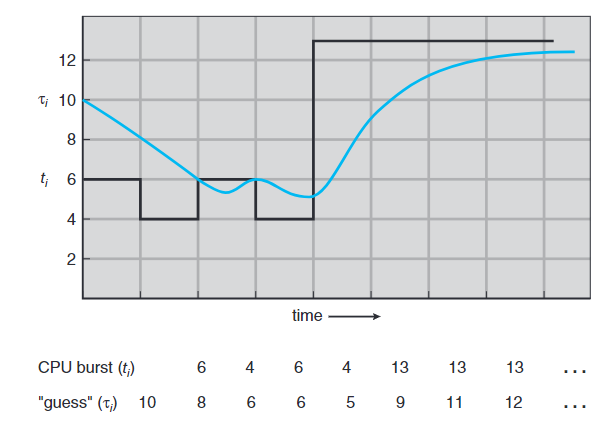
\includegraphics[width=0.309\textwidth]{pic/OS5/Prediction of the length of the next CPU burst}
    \caption{Prediction of the length of the next CPU burst}
\end{figure}


\subsubsection{Priority Scheduling}
smallest integer $\equiv$ highest priority. 

Problem: Starvation – low priority processes may never execute

Solution: Aging – as time progresses increase the priority of the process

相当于使用权重当作 burst time 估计的 SJF. 

\subsubsection{Round Robin (RR)}
Each process gets a small unit of CPU time (time quantum), usually 10-100 milliseconds. After this time has elapsed, the
process is preempted and added to the end of the ready queue. 

Performance:
\begin{itemize}
    \item $q$ large $\to$ FIFO
    \item $q$ small $\to$ $q$ must be large with respect to context switch,
    otherwise overhead is too high
\end{itemize}

\paragraph{Example of RR} with Time Quantum = 20
\begin{table}[!htb]
    \centering
    % \caption{}
    \begin{tabular}[c]{cc}\toprule
        Process & Burst Time \\ \midrule
        $P_1$ & 53 \\
        $P_2$ & 17 \\
        $P_3$ & 68 \\
        $P_4$ & 24 \\
        \bottomrule
    \end{tabular}
\end{table}

\begin{figure}[!htb]
    \centering
    \tikzmath{
        \step=0.8;
        \s1=0; 
        \s2=\step;
        \s3=\s2+\step;
        \s4=\s3+\step;
        \s5=\s4+\step;
        \s6=\s5+\step;
        \s7=\s6+\step;
        \s8=\s7+\step;
        \s9=\s8+\step;
        \ss1=\s9+\step;
        \ss2=\ss1+\step;
        \h=0.8;
    } 
    \begin{tikzpicture}
        \path[draw=black] (\s1,0) rectangle (\s2,\h);
        \path[draw=black] (\s2,0) rectangle (\s3,\h);
        \path[draw=black] (\s3,0) rectangle (\s4,\h);
        \path[draw=black] (\s4,0) rectangle (\s5,\h);
        \path[draw=black] (\s5,0) rectangle (\s6,\h);
        \path[draw=black] (\s6,0) rectangle (\s7,\h);
        \path[draw=black] (\s7,0) rectangle (\s8,\h);
        \path[draw=black] (\s8,0) rectangle (\s9,\h);
        \path[draw=black] (\s9,0) rectangle (\ss1,\h);
        \path[draw=black] (\ss1,0) rectangle (\ss2,\h);

        \node at (\s1/2 + \s2/2, \h/2) {$P_1$};
        \node at (\s2/2 + \s3/2, \h/2) {$P_2$};
        \node at (\s3/2 + \s4/2, \h/2) {$P_3$};
        \node at (\s4/2 + \s5/2, \h/2) {$P_4$};
        \node at (\s5/2 + \s6/2, \h/2) {$P_1$};
        \node at (\s6/2 + \s7/2, \h/2) {$P_3$};
        \node at (\s7/2 + \s8/2, \h/2) {$P_4$};
        \node at (\s8/2 + \s9/2, \h/2) {$P_1$};
        \node at (\s9/2 + \ss1/2, \h/2) {$P_3$};
        \node at (\ss1/2 + \ss2/2, \h/2) {$P_3$};

        \node at (\s1, -\h/2) {0};
        \node at (\s2, -\h/2) {20};
        \node at (\s3, -\h/2) {37};
        \node at (\s4, -\h/2) {57};
        \node at (\s5, -\h/2) {77};
        \node at (\s6, -\h/2) {97};
        \node at (\s7, -\h/2) {117};
        \node at (\s8, -\h/2) {121};
        \node at (\s9, -\h/2) {134};
        \node at (\ss1, -\h/2) {154};
        \node at (\ss2, -\h/2) {162};
    \end{tikzpicture}
    \caption{RR Example}
\end{figure}

平均等待时间更长, 但响应更好. 

\subsubsection{Multilevel Queue}
Ready queue is partitioned into separate queues:
\begin{itemize}
    \item foreground (interactive)
    \item background (batch)
\end{itemize}

Each queue has its own scheduling algorithm. Scheduling must be done between the queues. 

\begin{figure}[!htb]
    \centering
    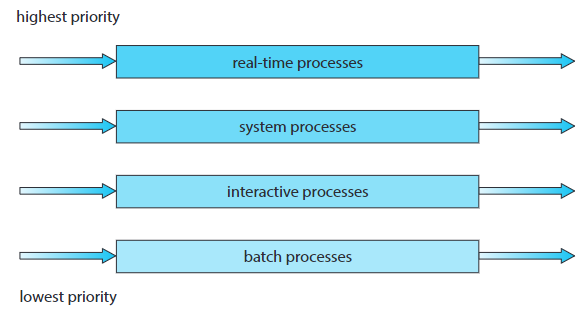
\includegraphics[width=0.42\textwidth]{pic/OS5/Multilevel queue scheduling}
    \caption{Multilevel queue scheduling}
\end{figure}


\subsubsection{Multilevel Feedback Queue}
A process can move between the various queues; aging can be implemented this way

Multilevel-feedback-queue scheduler defined by the following parameters:
\begin{enumerate}\small
    \item number of queues
    \item scheduling algorithms for each queue
    \item method used to determine when to upgrade a process
    \item method used to determine when to demote a process
    \item method used to determine which queue a process will enter when that process needs service    
\end{enumerate}

\paragraph{Example}Three queues:
\begin{enumerate}
    \item $Q_0$: RR with time quantum 8 milliseconds
    \item $Q_1$: RR time quantum 16 milliseconds
    \item $Q_2$: FCFS
\end{enumerate}

Scheduling:
\begin{itemize}\small
    \item A new job enters queue $Q_0$ which is served FCFS. When it
    gains CPU, job receives 8 milliseconds. If it does not finish in 8
    milliseconds, job is moved to queue $Q_1$.
    \item At $Q_1$ job is again served FCFS and receives 16 additional
    milliseconds. If it still does not complete, it is preempted and
    moved to queue $Q_2$.    
\end{itemize}

\begin{figure}[!htb]
    \centering
    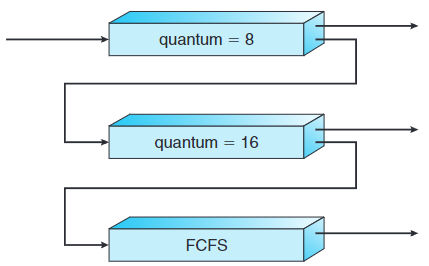
\includegraphics[width=0.309\textwidth]{pic/OS5/Multilevel feedback queues}
    \caption{Multilevel feedback queues}
\end{figure}

\subsection{Multiple-Processor Scheduling}
\begin{itemize}\small
    \item Asymmetric multiprocessing: 只有一个处理器访问系统数据结构, 从而减轻了对数据共享的需要; 其他人只执行用户代码.
    \item Symmetric multiprocessing (SMP): 每个处理器都是自调度的. 多个处理器可能访问和更新一个公共数据结构. 
\end{itemize}

\subsection{Real-Time Scheduling}
\begin{itemize}\small
    \item Hard real-time systems: 在保证的时间内完成所需关键任务
    \item Soft real-time computing: 要求关键流程优先于其他的流程
\end{itemize}

\subsection{Thread Scheduling}
Also known as the Contention Scope. 
\begin{itemize}\small
    \item Local Scheduling (Process-Contention Scope): 线程库如何决定将哪个线程放入可用的LWP
    \item Global Scheduling (System-Contention Scope): 内核如何决定下一个运行的内核线程
\end{itemize}

